\documentclass[titlepage,a4paper,oneside]{article}
\usepackage[utf8]{inputenc}
\usepackage{amsmath}
\usepackage{amssymb}
\usepackage{mathabx}
\usepackage{adjustbox}
\usepackage{graphicx}
\usepackage{minted}
\usepackage{booktabs}
\usepackage[english,spanish,es-noindentfirst,es-nosectiondot,es-nolists,
es-noshorthands,es-lcroman,es-tabla]{babel}
\usepackage{lmodern}             % Use Latin Modern fonts
\usepackage[T1]{fontenc}         % Better output when a diacritic/accent is used
\usepackage[utf8]{inputenc}      % Allows to input accented characters
\usepackage{textcomp}            % Avoid conflicts with siunitx and microtype
\usepackage{microtype}           % Improves justification and typography
\usepackage[svgnames,table,xcdraw]{xcolor}    % Svgnames option loads navy (blue) colour
\usepackage[hidelinks,urlcolor=blue]{hyperref}
\hypersetup{colorlinks=true, allcolors=Navy, pdfstartview={XYZ null null 1}}
\newtheorem{lemma}{Lema}
\usepackage[width=14cm,left=3.5cm,marginparwidth=3cm,marginparsep=0.35cm,
height=21cm,top=1.7cm,headsep=1cm, headheight=1.6cm, footskip=1.2cm, bottom=1.4cm]{geometry}
\usepackage{csquotes}
\usepackage{mathrsfs}
\usepackage{biblatex}
\addbibresource{informe.bib}
\usepackage[pdf]{graphviz}

\begin{document}

\begin{titlepage}
\title{
	75.26 \-- Simulación \\
    \large Facultad de Ingeniería\\
	Universidad de Buenos Aires
}
\author{
	Mermet, Ignacio Javier\\
	\texttt{98153}
}
\date{Julio 2023}

\maketitle

\end{titlepage}

\tableofcontents

\newpage

\section{Introducción}
En el presente trabajo se hará una Introducción al paper \textit{Beyond Finite Layer Neural Networks: Bridging Deep Architectures and Numerical Differential Equations}\cite{lu18d} de \textit{Lu et. al}.  Se introduce la motivación de los autores, una breve reseña de la literatura para explicar el estado del arte en el momento de publicación, se explican los puntos principales del paper y mostramos los resultados obtenidos al intentar replicar los resultados obtenidos en el paper.

\subsection{Entrenamiento de redes neuronales muy profundas}
Las redes neuronales convolucionales empezaron a dominar el campo de vision por computadora luego de la introducción de AlexNet \cite{DBLP:journals/corr/Krizhevsky14} en 2012. Una gran ventaja de esta familia de modelos es que aprenden mapas de \textit{features} junto con un clasificador en un proceso punta a punta. De este modo, no es necesario que se definan a priori las \textit{features} relevantes de la imagen o del dominio bajo estudio.

Desde entonces, se ha acelerado el estudio de estas familias de modelos, con aplicaciones varias en imágenes, lenguaje natural, sonido, procesamiento de señales, sistemas de recomendaciones, entre otras. Distintos papers elaboran sobre la importancia de la profundidad de dichas redes para lograr mejores resultados. Es decir, la performance, bajo alguna medida de performance relevante al problema, aumenta al agregar capas de parámetros libres o bloques con más neuronas. Sin embargo, el entrenamiento de modelos cada vez más grandes ha expuesto varios problemas relacionados a la convergencia del entrenamiento.

Un problema común a la hora de entrenar redes neuronales muy profundas es la explosión de gradientes, otro es el desvanecimiento de gradientes. El primero se refiere a que los valores de los gradientes a medida que se propagan por la red toman valores exponencialmente más grandes, hasta tomar el valor nan. De este valor, no se pueden recuperar, dado que las operaciones de matmul no se encuentran definidas. El segundo se refiere al caso contrario, donde los gradientes se vuelven progresivamente más pequeños y tienden a cero, frenando por completo el entrenamiento. En ambos casos, la convergencia de la red se ve afectada. Ambos problemas se hacen más aparentes en redes neuronales muy profundas. Estos problemas han sido, a grandes rasgos, resueltos mediante el uso de distintos métodos de regularización entre capas así como de inicialización normalizada.

Sin embargo, aún convergiendo, una consecuencia de aumentar la profundidad de las redes, es que se evidencia una degradación en el error de aprendizaje. La precisión de la red se satura y luego empeora. Sería natural que se trata de un caso de sobreajuste u \textit{overfitting}, pero no es el caso.


\subsection{Redes residuales}
Dentro de la literatura que trata de ajustar este problema, \cite{DBLP:journals/corr/HeZRS15} propone lo que denomina aprendizaje de residuos para resolver el problema de degradación. En esta sección hago un breve resumen de \S 1 del paper de ResNet a fin de proveer el contexto necesario para el resto de esta monografía.

\begin{figure}[H]
\centering
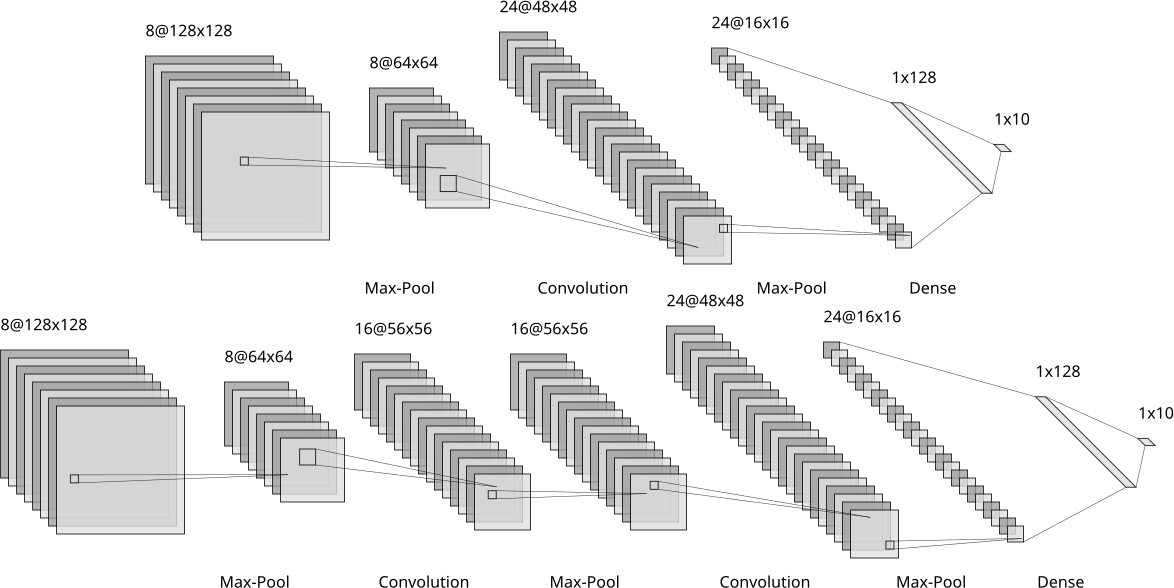
\includegraphics[width=\textwidth]{images/ex_cnns.png}
\caption{Ejemplo de CNNs}
\label{ex_cnn}
\end{figure}

La segunda CNN en \ref{ex_cnn} posee una capa mas de conv-maxpooling que la primera. Asumamos que las demás capas están copiadas de la primer CNN de la figura, con sus mismos pesos. La capa extra podría aprender un mapeo de identidad y por tanto tener \textit{al menos} la misma precisión que la primer CNN de la figura. Esta solución por construcción de una red efectivamente más profunda indicaría que una red más profunda debería tener un error de entrenamiento más chico que una red más chica, pero esto se contradice con distintos resultados experimentales.

En lugar de esperar que algún conjunto de capas aprendan un mapeo deseado, se les hace aprender un mapeo residual: deseando aprender el mapeo $\mathscr{H}(x)$, dejan que ese conjunto no lineal de capas aprenda $\mathscr{F}(x) = \mathscr{H}(x) - x$, de modo de obtener la función original como $\mathscr{F}(x) + x$. Los autores conjeturan que es más fácil optimizar el mapeo residual que el mapeo original. Volviendo a nuestro argumento de construcción, si el mapeo identidad fuera óptimo, sería más facil llevar el residual a cero que aprender $\mathscr{H}(x)$ como un mapeo de identidad.

Dicha formulación puede ser expresada como conexiones entre capas no contiguas de una red neuronal. ResNet utiliza mapeos identidad como conexiones de "atajo" entre capas (\ref{resnet_block}), dado que no introducen costo computacional extra ni agregan parámetros libres a la red. La salida de estas conexiones simplemente se suma a la salida de la capa. De este modo, se puede optimizar por backpropagation. En \ref{resnet_torch} se ilustra su implementación utilizando \texttt{pytorch}.

\begin{figure}[H]
\centering
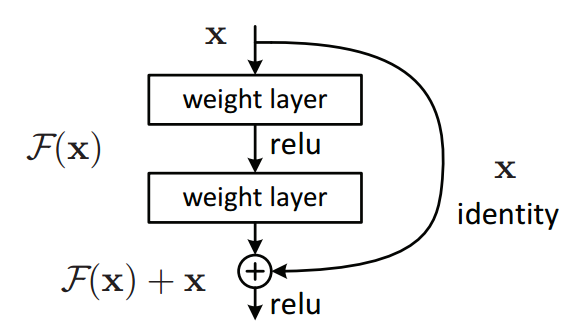
\includegraphics[scale=0.5]{images/resnet_block.png}
\caption{Bloque de ResNet}
\label{resnet_block}
\end{figure}


\begin{figure}[H]
\begin{minted}[mathescape,
               linenos,
               numbersep=5pt,
               gobble=0,
               frame=lines,
               framesep=2mm,
	       firstnumber=1]{python}
class ResidualBlock(nn.Module):
    def __init__(
        self,
        in_channels: int,
        out_channels: int | None = None,
        stride: int = 1,
        kernel_size: int = 3,
        padding: int = 1,
        downsampling: bool = False,
    ):
        super().__init__()

        if out_channels is None:
            out_channels = in_channels

        self.downsampling = downsampling

        self.main_block = nn.Sequential(
            nn.Conv2d(
                in_channels,
                out_channels,
                kernel_size=kernel_size,
                stride=stride,
                padding=padding,
            ),
            nn.BatchNorm2d(out_channels),
            nn.ReLU(),
            nn.Conv2d(
                out_channels,
                out_channels,
                kernel_size=kernel_size,
                # stride=stride,
                padding=padding,
            ),
            nn.BatchNorm2d(out_channels),
        )

        if not downsampling:
            self.res_f = nn.Identity()
        else:
            self.res_f = nn.Sequential(
                nn.Conv2d(
                    in_channels,
                    out_channels,
                    kernel_size=1,
                    stride=stride,
                    # padding=padding,
                ),
                nn.BatchNorm2d(out_channels),
            )

    def forward(self, x):
        residual = x
        out = self.main_block(x)
        residual = self.res_f(residual)
        out += residual
        out = F.relu(out)
        return out
\end{minted}
\label{resnet_torch}
\caption{Ejemplo de implementación con \texttt{pytorch} de un bloque residual.}
\end{figure}

Al implementar esta arquitectura, se muestran resultados experimentales que indican que:
\begin{itemize}
	\item Arquitecturas de redes residuales muy profundas son fácilmente optimizables
	\item El error de sus contrapartes no residuales aumenta conforme aumenta su profundidad
	\item Las redes residuales pueden aumentar su precisión simplemente agregando más bloques
\end{itemize}

\section{Arquitecturas residuales como sistemas dinámicos}
Observemos, brevemente, que cada bloque residual de ResNet puede ser descrito por el siguiente sistema dinamico discreto \cite{E-2017}:

\begin{align}\label{ODE_ResNet}
	    y_l &= h(z_l) + \mathscr{F}(z_l, W_l)\\
	y_{l+1} &= g(y_l)
\end{align}

Donde $z_l$ es la entrada del l-ésima capa, $z_{l+1}$ es la salida de la l-ésima capa, $y_l$ es una variable auxiliar de la l-ésima capa, $h, g$ son mapeos que pueden ser no-lineales. El entrenamiento, experimentalemente, se determina \cite{he2016identity} que es más facil si sendos $g$ y $h$ son el mapa identidad.

Consideremos $G$ como la inversa de $g$, entonces el sistema dinamico anterior puede ser descrito como

\begin{align}\label{ODE23}
	z_{l+1} = G(h(z_l) + \mathscr{F}(z_l, W_l))
\end{align}

Para que el sistema sea estable (no haya desvanecimiento o explosión de gradientes), el gradiente del lado derecho debe ser cercano a la identidad. Asumiendo $\mathscr{F}$ como una pequeña perturbación, entonces se requiere que $\nabla G \nabla h \approx I$, lo cual se cumple si $g$ y $h$ son mapas identidad. En tal caso, \ref{ODE23} se convierte en:

\begin{align}
	z_{l+1} = z_l + \mathscr{F}(z_l, W_l)
\end{align}

Lo cual se puede ver como una discretización del sistema dinámico

\begin{align}
	\dfrac{dz}{dt} = \mathscr{F}(z, W(t))
\end{align}

Cuya discretización más sencilla toma la forma

\begin{align}
	z_{l+1} = z_l + \Delta t_l \mathscr{F}(z_l, W_l)
\end{align}

Donde $\Delta t_l$ es el tamaño del l-ésimo paso. Notemos que esto es el primer paso del método de Euler.

\subsubsection{PolyNet}
En \cite{szegedy2014going}, se propone una arquitectura llamada "Inception" cuyos bloques se muestran en \ref{inception_block}.

\begin{figure}[H]
\centering
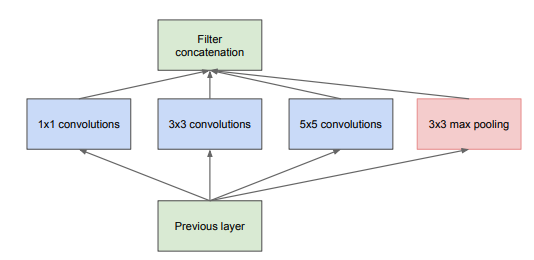
\includegraphics[height=200px]{images/inception_block.png}
\caption{Bloque de Inception}
\label{inception_block}
\end{figure}

Zhang et al proponen en \cite{zhang2017polynet} utilizar bloques de Inception como bloques residuales. En \ref{polynet_block} se muestra el diagrama original.

\begin{figure}[H]
\centering
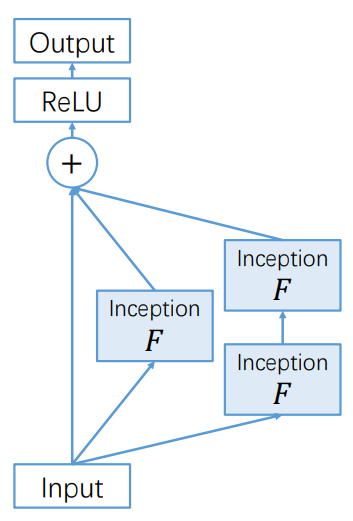
\includegraphics[height=200px]{images/polynet.png}
\caption{Bloque de PolyNet}
\label{polynet_block}
\end{figure}

Es necesario aclarar que todos los bloques etiquetados "Inception F" comparten sus parámetros. Configuraciones donde distintos bloques no comparten parámetros son también estudiadas. La motivación principal es estudiar composiciones polinomiales de operadores para explorar la diversidad estructural que permite combinar aditivamente distintos bloques.

Notar que esto resulta en un término de segundo orden respecto de ResNet.

\begin{align}\label{PolyNet_ODE}
	(I + F + F^2) \cdot x &= x + F(x) + F(F(x))
\end{align}

Cuyo lado izquierdo puede reescribirse como
\begin{align}
	I + (I + F) F  = I + F + F^2
\end{align}

De modo tal que su computo sea mas eficiente.

Esta formulación puede verse como un paso del método implicito de Euler

\begin{align}
	u_{n+1} = (I -\Delta tf)^{-1}u_n
\end{align}

Para la ecuación diferencial $u_t = f(u)$. El método implicito permite pasos mas grandes, de modo que son necesarios menos bloques encadenados para lograr clasificación de estado del arte.

\subsubsection{FractalNet}
FractalNet \cite{larsson2017fractalnet} muestra que el aprendizaje explicito de residuales no es un imperativo para entrenar redes muy profundas.

\begin{figure}[H]
\centering
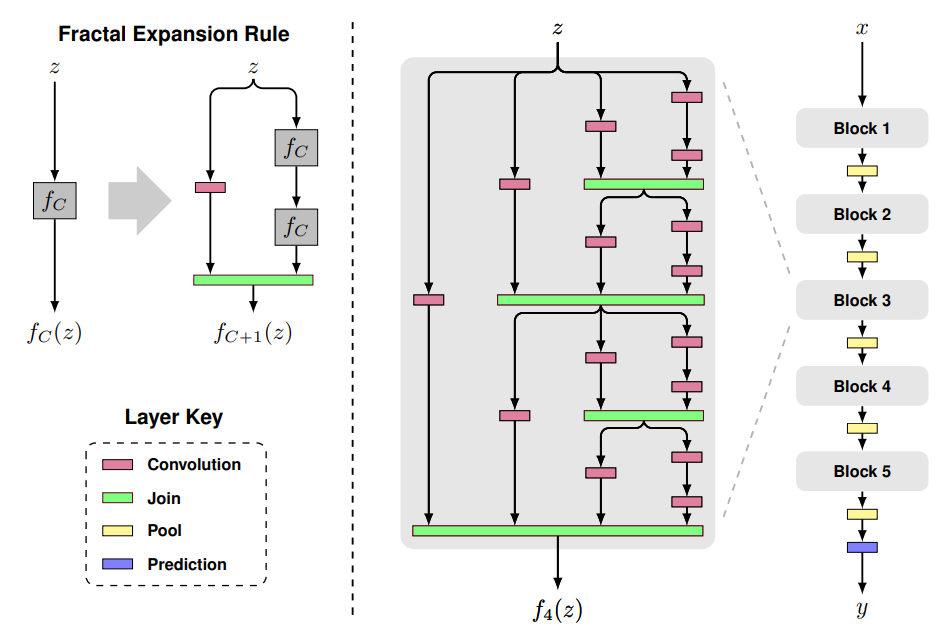
\includegraphics[width=\textwidth]{images/fractal_expansion.png}
\caption{Regla de expansión de FractalNet}
\label{fractal_expansion}
\end{figure}

\ref{fractal_expansion} muestra la regla de expansión de FractalNet. Siendo C el indice de un fractal truncado $f_C(\cdot)$, la estructura de FractalNet esta definida por $f_C(\cdot)$. El caso base se define como una red con una sola capa convolucional: $f_1(z) = \text{conv}(z)$.

Los fractales sucesivos se definen como

\begin{align}\label{fractal_net_eq}
	f_{C+1}(z) = \left[ (f_C \circ f_C)(z) \right] \oplus \left[ \text{conv}(z) \right]
\end{align}

Donde $\circ$ denota composicion de funciones y $\oplus$ un operador de unión. Este operador de unión puede ser, por ejemplo, concatenación o suma elemento a elemento. Los autores utilizan el promedio elemento a elemento.

Entonces, \ref{fractal_net_eq} puede ser reescrito como:

\begin{align}
	f_{c+1} = \dfrac{1}{2} f_c \circ f_c + \dfrac{1}{2} k_c
\end{align}

Entonces, cada bloque de FractalNet de orden dos puede ser reescrito como:

\begin{align}
	x_{n+1} = k_1 \times x_n + k_2 \times (k_3 \times x_n + f_1(x_n)) + f_2 (k_3 \times x_n + f_1(x_n))
\end{align}

Lo cual puede ser considerado como un caso de un esquema de Runge-Kutta de segundo orden para la EDO $u_t = f(u,t)$.

\subsubsection{RevNet}
Recordemos que un sistema dinamico es reversible si su función de transición de estados es biyectiva. Es decir, para cada estado existe un unico estado anterior desde el cual podría haberse llegado.

En \cite{gomez2017reversible} se propone RevNet, una arquitectura compuesta de una serie de bloques reversibles. Los parámetros de cada capa se particionan en dos grupos $x_1, x_2$. Cada bloque reversible toma dos entradas $(x_1, x_2)$ y produce dos salidas $(y_1, y_2)$ acorde a las reglas en \ref{eq_revnet} y funciones residuales $\mathscr{F}$ y $\mathscr{G}$ analogas a ResNet.

\begin{align}\label{eq_revnet}
	y_1 &= x_1 + \mathscr{F}(x_2) \\
	y_2 &= x_2 + \mathscr{G}(y_1)
\end{align}

Por tanto, las activaciones de una capa pueden ser reconstruidas desde las activaciones de la próxima capa:

\begin{align}
	x_2 &= y_2 - \mathscr{G}(y_1) \\
	x_1 &= y_1 - \mathscr{F}(x_2)
\end{align}

De este modo, se ejecuta backpropagation sin guardar las activaciones en memoria.\footnote{La VRAM en GPUs suele ser un limitante en el entrenamiento. Si la arquitectura tiene muchos parámetros, es común utilizar un batch size más chico, lo cual es subóptimo para SGD con mini batches.} De este modo, su costo en memoria es independiente de su profundidad, a excepción de algunas pocas capas no reversibles.

Reformulemos \ref{eq_revnet} como el siguiente sistema dinamico discreto:

\begin{align}
	X_{n+1} &= X_n + \mathscr{F}(Y_n) \\
	Y_{n+1} &= Y_n + \mathscr{G}(X_{n+1})
\end{align}

Con lo cual podemos apreciar su interpretación como un paso del método de Euler del sistema dinámico:

\begin{align}
	\dot{X} &= f_1(Y, t) \\
	\dot{Y} &= f_2(X, t)
\end{align}

\subsection{LM-ResNet}
Notemos que todas las formulaciones anteriores se corresponden con métodos de un solo paso para aproximar sistemas dinámicos. En \cite{lu18d} proponen una arquitectura basada en el método lineal de múltiples pasos.

\subsubsection{Métodos multipasos}
Los métodos de Euler y Runge Kutta mencionados previamente requieren solamente conocer el valor de $y_i$ para poder calcular $y_{i+1}$. En un método multi pasos, se emplean dos o más puntos anteriores para calcular el siguiente punto.

Dado un problema a valores iniciales

\begin{equation}
\left\{ \begin{aligned}
		y\prime &= f(t,y), \enspace a \leq t \leq b\\
		y(a) &= \alpha
\end{aligned} \right.
\end{equation}

Un método multi pasos de orden $m > 1$ es aquel cuya ecuación en diferencias para aproximar $y_{i+1}$ en $t_{i+1}$ se corresponde con la ecuación:

\begin{align}
	y_{i+1} &= a_{m-1} y_i + a_{m-2} y_{i-1} + \ldots + a_0 y_{i+1-m} \\
	        &+ h \left[b_m f(t_{i+1}, y_{i+1}) + b_{m-1} f(t_i, y_i) + \ldots + b_0 f(t_{i+1-m}, y_{i+1-m})  \right]
\end{align}

Con $i=m-1, m, \cdots, N-1$ y donde $a_0, a_1, \cdots, a_{m-1}$ y $b_0, b_1, \cdots, b_m$ son constantes y los valores iniciales $y_0 = \alpha, y_1 = \alpha_1, y_2 = \alpha_2, \cdots, y_{m-1} = \alpha_{m-1}$ son especificados.

Si $b_m = 0$, el método es \textbf{explícito o abierto} ya que el valor de $w_{i+1}$ se da explícitamente en términos de los valores previamente calculados. Cuando $b_m \neq 0$, el método es \textbf{implícito o cerrado}, ya que el valor de $w_{i+1}$ se encuentra en ambos miembros de la ecuación y se especifica sólo implicitamente.

\subsubsection{Formulación de LM-ResNet}
La arquitectura LM puede ser formulada como

\begin{align}\label{LM_arch}
	u_{n+1} = (1-k_n) u_n + k_n u_{n-1} + f_n(u_n)
\end{align}

Donde $k_n \in \mathbb{R}^n$ es un paramétro entrenable de cada capa que actúa como factor de escalado del residuo de la capa actual y la anterior. La figura \ref{lmblock} muestra el bloque de LM-ResNet \textit{acorde al código original}. Notar que \ref{lmblockorig}, el bloque según el paper, presenta diferencias. En primer instancia, el código original multiplica el residuo de la capa previa por $1-k_s$, pero acorde a la ecuación \ref{LM_arch}, y el diagrama \ref{lmblockorig}, se multiplica por $k_s$. El diagrama original es poco claro también, pareciendo indicar que se multiplica $u_n$ tanto por $k_s$ como por $1-k_s$.

\begin{figure}[H]
\centering
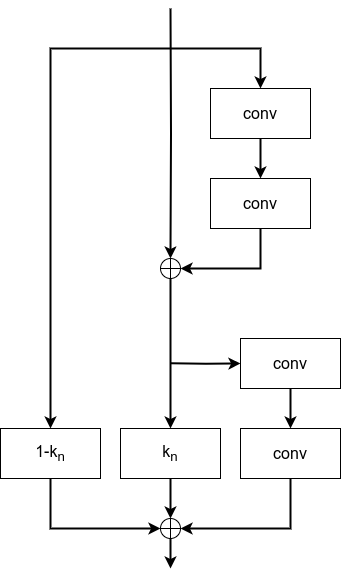
\includegraphics[height=200px]{images/LM-Block.png}
\caption{Bloque de LM-ResNet}
\label{lmblock}
\end{figure}

\begin{figure}[H]
\centering
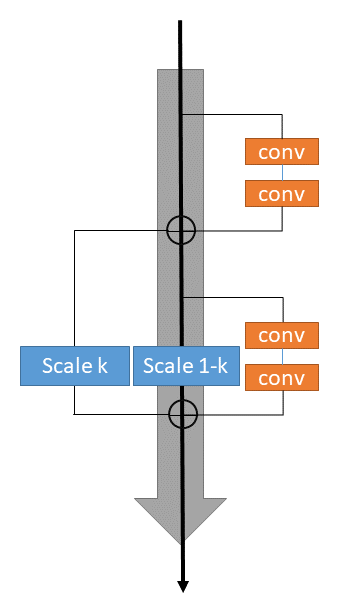
\includegraphics[height=200px]{images/LM-Block-orig.png}
\caption{Bloque de LM-ResNet, acorde al paper original.}
\label{lmblockorig}
\end{figure}

Para los resultados experimentales, se toma como verdad el código. Por tanto, debemos modificar \ref{LM_arch} acordemente como:

\begin{align}
	u_{n+1} = f_n(u_n) + k_n \times u_n + (1-k_n) \times u_{n-1}
\end{align}

\section{Resultados experimentales}
En esta sección se detallan los resultados de distintos experimentos desarrollados a fin de replicar los resultados expuestos en el paper. A estos efectos, se utiliza el código original y se arma un pipeline de entrenamiento acorde a lo relatado en el paper.

\subsection{CIFAR10}
Los experimentos aquí detallados se realizan utilizando el dataset CIFAR10. Este dataset se compone de 60000 imágenes de 32x32 píxeles con tres canales de color (RGB). Se divide en 50000 imágenes de entrenamiento y 10000 para el set de pruebas.

Siguiendo lo especificado en \S 2.2, se aplican técnicas de image augmentation al dataset de entrenamiento. TODO. En particular, se agrega un padding de 4 píxeles a cada lado, de modo tal que la imagen pasa a tener 40x40 píxeles. Con una probabilidad del 50\% se espeja la imagen horizontalmente. Finalmente, se toma un recorte aleatorio de 32x32 píxeles.

En etapa de pruebas, se toma una vista simple de la imagen original de 32x32. Es importante notar esto dado que el paper de ResNet utiliza otra técnica de evaluación, tomando múltiples vistas de la imagen original.

\subsection{Hiperparámetros relevantes}
A fin de seguir los lineamientos planteados por el paper, se modificó el código original y se implementó un pipeline de entrenamiento con los hiperparámetros especificados. El batch size se configuró como 128 imágenes por batch. Se utiliza SGD como optimizador, con weight decay  configurado como 0.0001 y momentum como 0.9. En \ref{lrcurve} se especifica la curva del parametro de learning rate.

\begin{figure}[H]
\centering
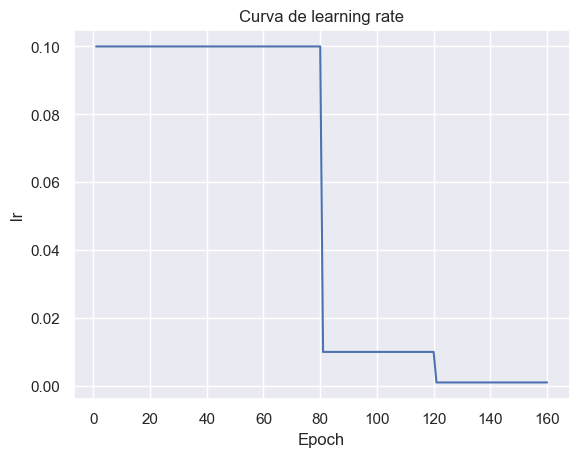
\includegraphics[width=\textwidth]{images/lr_curve.png}
\caption{Curva de learning rate}
\label{lrcurve}
\end{figure}

El entrenamiento se detiene a los 160 epochs.

Todos los experimentos fueron llevados a cabo con CUDA 12.1 en una GPU Nvidia 2070 Super con 8GB de memoria de video.

\subsection{Resultados}

% Please add the following required packages to your document preamble:
% \usepackage[table,xcdraw]{xcolor}
% If you use beamer only pass "xcolor=table" option, i.e. \documentclass[xcolor=table]{beamer}
\begin{table}[H]
\begin{adjustbox}{center}
\begin{tabular}{l|ll|ll|lll|}
\cline{2-8}
 & \multicolumn{2}{c|}{\textbf{Replicación}} & \multicolumn{2}{c|}{\textbf{Paper}} &  &  &  \\ \cline{2-8}
 & \multicolumn{1}{c}{\textbf{Acc.}} & \multicolumn{1}{c|}{\textbf{Error (\%)}} & \multicolumn{1}{c}{\textbf{Acc.}} & \multicolumn{1}{c|}{\textbf{Error (\%)}} & \multicolumn{1}{c|}{\textbf{\begin{tabular}[c]{@{}c@{}}Diferencia\\ de error\end{tabular}}} & \multicolumn{1}{l|}{\textbf{\begin{tabular}[c]{@{}l@{}}Parametros\\ entrenables\end{tabular}}} & \textbf{\begin{tabular}[c]{@{}l@{}}Mult-Add\\ totales (G)\end{tabular}} \\ \hline
\multicolumn{1}{|l|}{\textbf{MResNet-20}} & 0.9189 & 8.11 & 0.9167 & 8.33 & \multicolumn{1}{l|}{\cellcolor[HTML]{77DD77}+0.22} & \multicolumn{1}{l|}{273475} & 5.22 \\
\multicolumn{1}{|l|}{\textbf{MResNet-32}} & 0.9263 & 7.37 & 0.9282 & 7.18 & \multicolumn{1}{l|}{\cellcolor[HTML]{FF6961}-0.19} & \multicolumn{1}{l|}{467913} & 8.85 \\
\multicolumn{1}{|l|}{\textbf{MResNet-44}} & 0.9296 & 7.04 & 0.9334 & 6.66 & \multicolumn{1}{l|}{\cellcolor[HTML]{FF6961}-0.38} & \multicolumn{1}{l|}{662351} & 12.47 \\
\multicolumn{1}{|l|}{\textbf{MResNet-56}} & 0.9316 & 6.84 & 0.9369 & 6.31 & \multicolumn{1}{l|}{\cellcolor[HTML]{FF6961}-0.53} & \multicolumn{1}{l|}{856789} & 16.10 \\
\multicolumn{1}{|l|}{\textbf{MResNet-110}} & 0.9350 & 6.5 & 0.9384 & 6.16 & \multicolumn{1}{l|}{\cellcolor[HTML]{FF6961}-0.34} & \multicolumn{1}{l|}{1731760} & 32.40 \\
\multicolumn{1}{|l|}{\textbf{MResNet-164}} & 0.9474 & 5.26 & 0.9473 & 5.27 & \multicolumn{1}{l|}{\cellcolor[HTML]{77DD77}+0.1} & \multicolumn{1}{l|}{1703760} & 31.70 \\ \hline
\end{tabular}
\caption{Tabla de resumen de resultados obtenidos.}
\end{adjustbox}
\end{table}


TODO Diferencia hiperparametros

\begin{figure}[H]
\centering
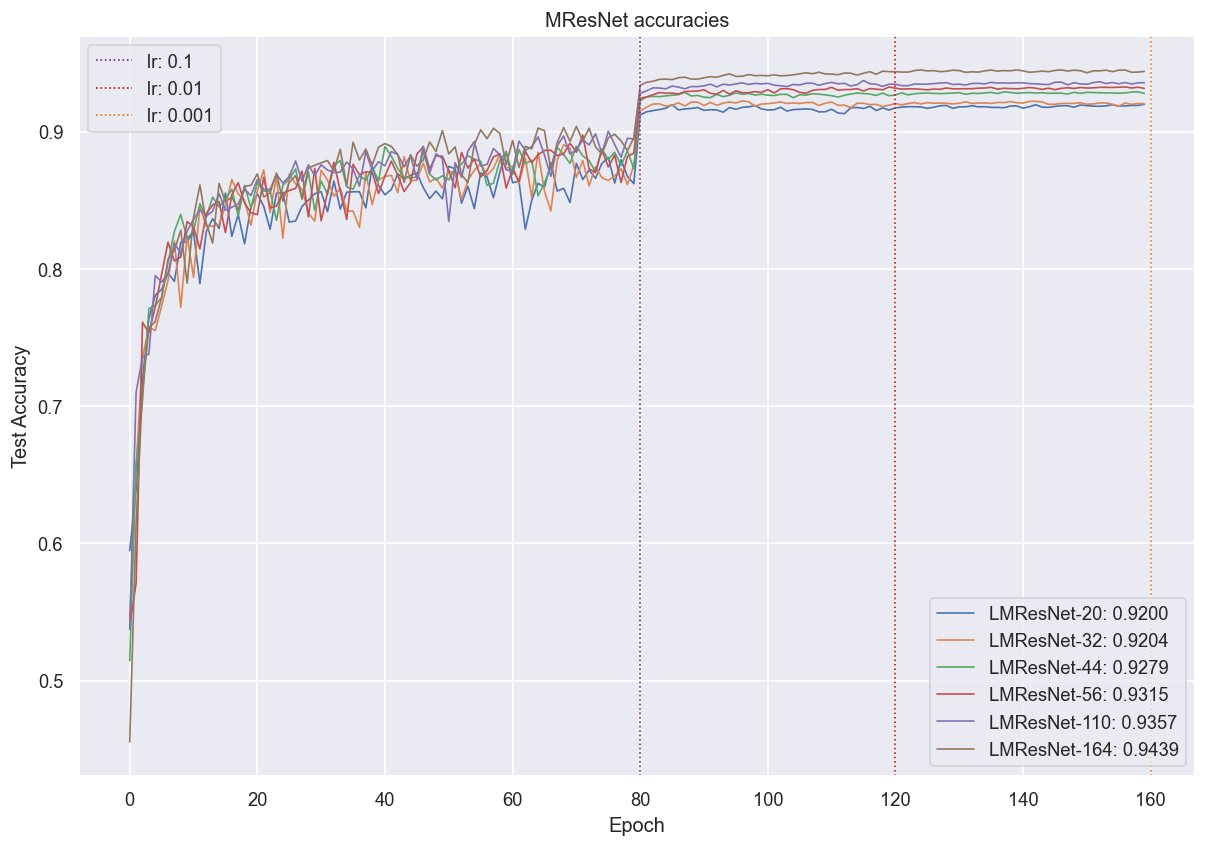
\includegraphics[width=\textwidth]{images/accuracy.png}
\caption{Accuracy sobre el set de test}
\label{test_set_acc}
\end{figure}

\begin{figure}[H]
\centering
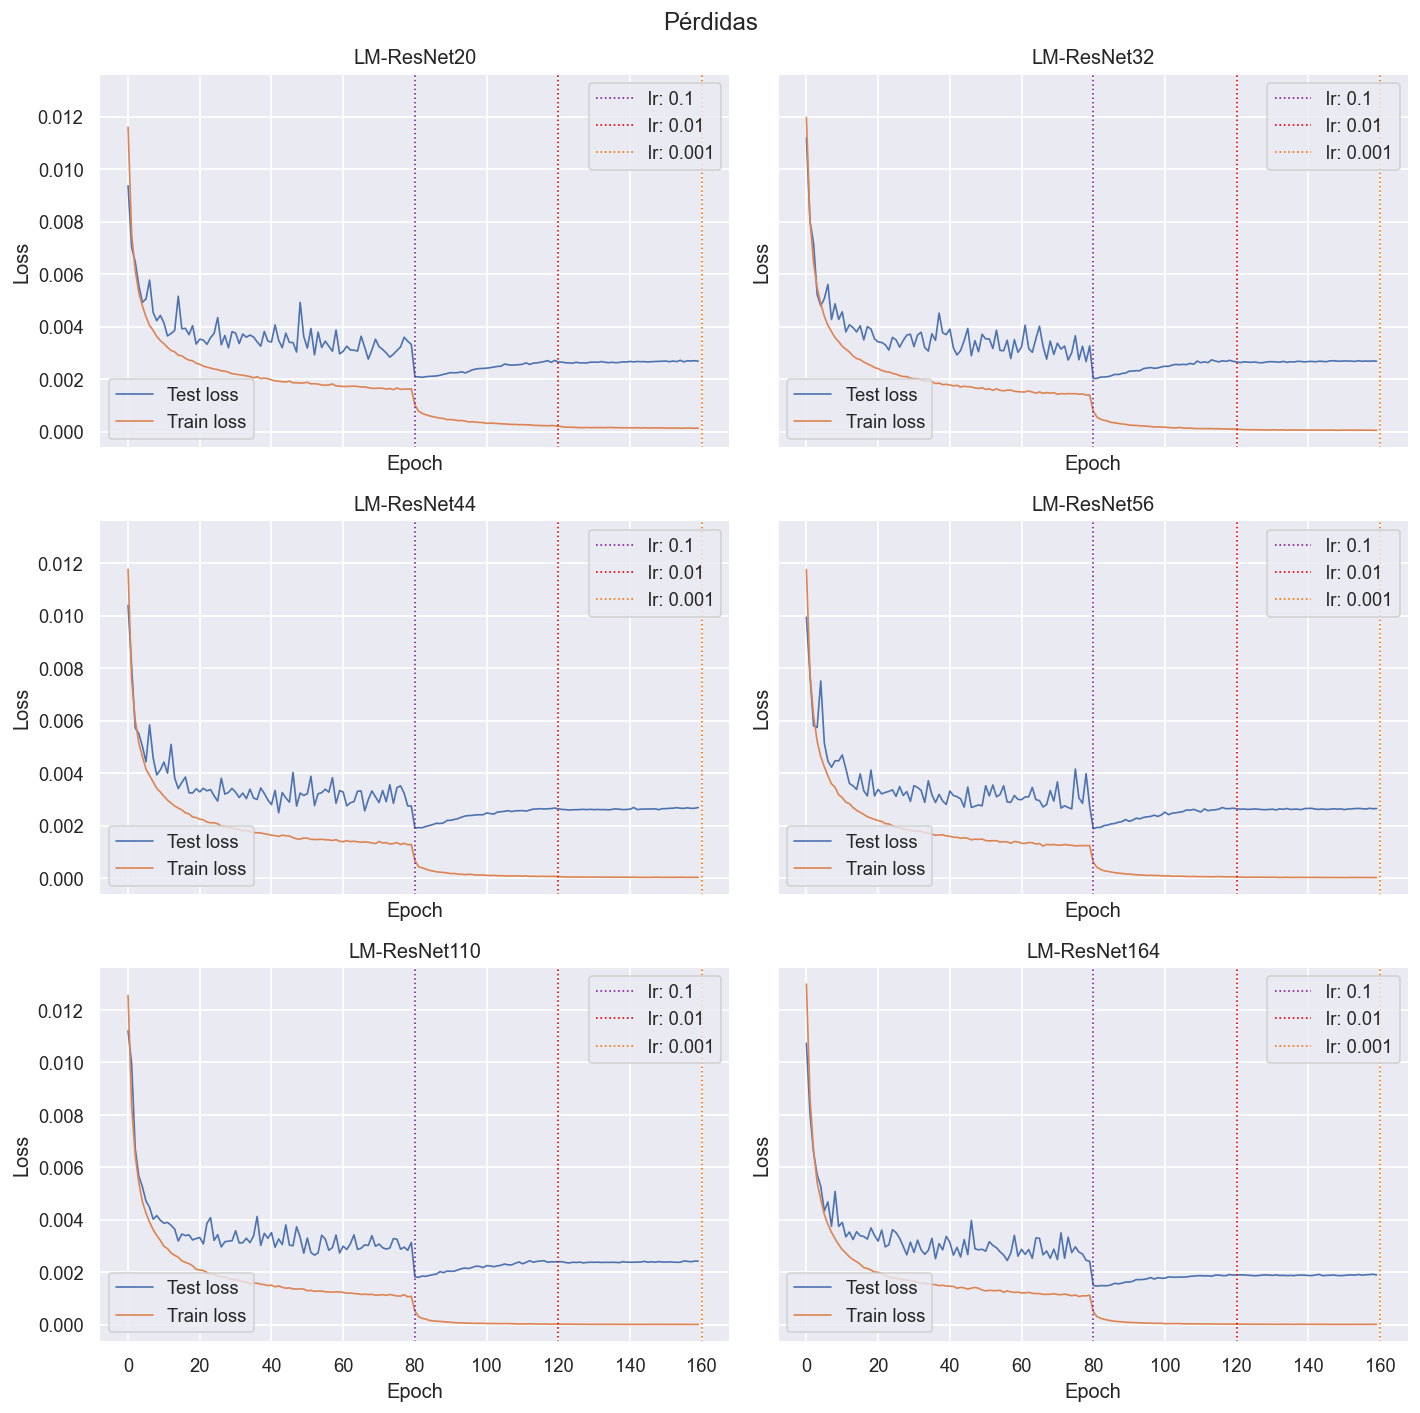
\includegraphics[width=\textwidth]{images/loss.png}
\caption{Pérdida (cross-entropy) de cada modelo durante entrenamiento}
\label{train_loss}
\end{figure}

\begin{figure}[H]
\centering
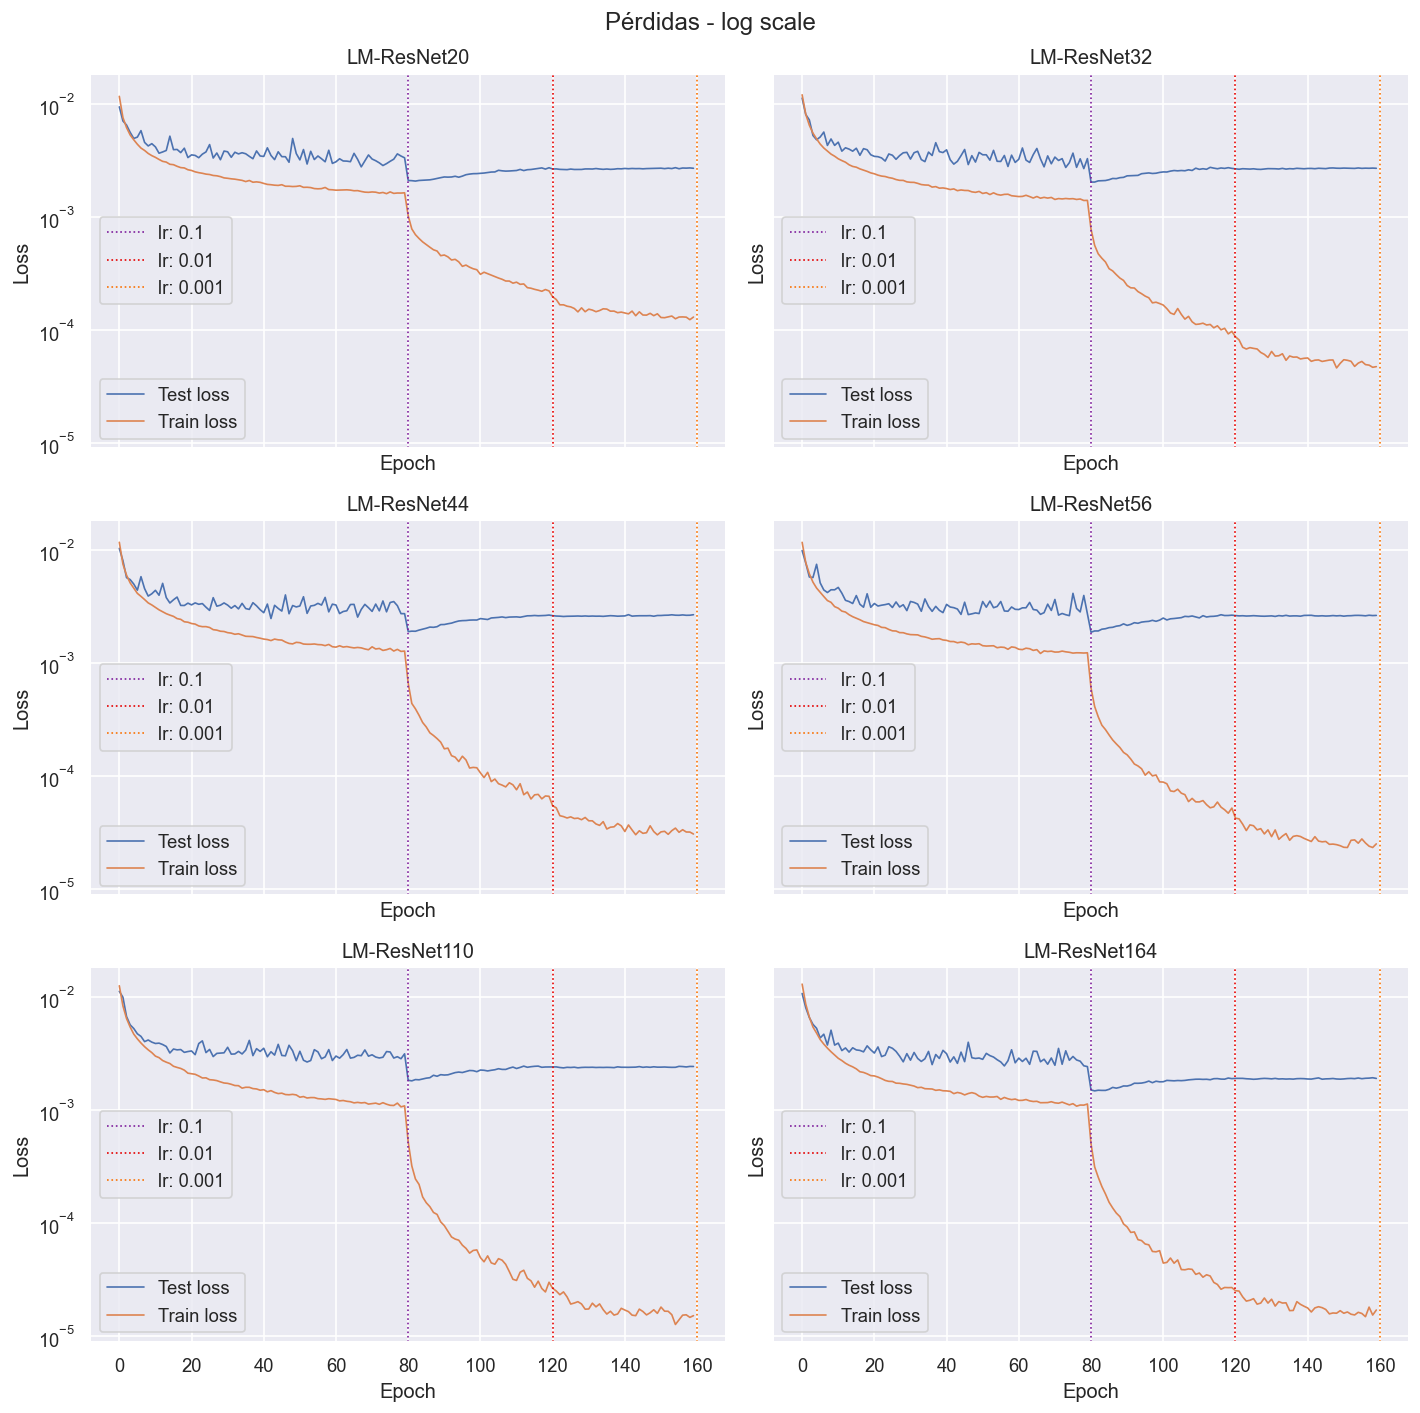
\includegraphics[width=\textwidth]{images/loss_log.png}
\caption{Pérdida (cross-entropy) de cada modelo durante entrenamiento. Escala logarítmica.}
\label{train_loss_log}
\end{figure}

\section{Sistemas dinámicos estocásticos}
En \cite{huang2016deep}, se propone, aleatoriamente eliminar un subset de capas y reemplazarlas por la función identidad. Se inicia con una red extremadamente profunda (incluso más de 1200 capas) para luego ir eliminando en entrenamiento. Por otro lado, \cite{gastaldi2017shakeshake} propone utilizar regularización shake-shake para mejorar los resultados de una red con múltiples ramas (como LM-Resnet), reemplazando la operación de suma como unión de ramas por una operación afín estocástica.

\subsection{Sistema dinámico de una regularización Shake-Shake}
Tal se adelantó, en \cite{gastaldi2017shakeshake},

\begin{align}
	X_{n+1} = X_n + \eta f_1(X_n) + (1-\eta) f_2 (X_n)
\end{align}

Describe la combinación afín estocástica de múltiples componentes de un bloque residual introducida. $\eta \sim \mathscr{U}(0,1)$. Introduciendo un paso temporal $\Delta t$ encontramos su sistema dinamico estocástico:

\begin{align}
	X_{n+1} = X_n + \left(\dfrac{\Delta t}{2} + \sqrt{\Delta t}(\eta - \dfrac{1}{2})\right) f_1(X_n) + \left( \dfrac{\Delta t}{2} + \sqrt{\Delta t} (\dfrac{1}{2} - \eta) \right) f_2(X_n)
\end{align}

Cuando $\Delta t \equiv 1$, la ecuación anterior se reduce a la regularización shake-shake. Podemos reescribir la

\section{Conclusión}
En el presente trabajo se explica el paper ``Beyond Finite Layer Neural Networks'', explicando el estado del arte previo, su motivación y los temas más relevantes de la literatura relacionada. Se implementan los pipelines de entrenamientos necesarios para replicar los resultados, reportamos la diferencia obtenida respecto de los resultados reportados en el paper. Se hacen notar varios problemas en el paper original y el código.

\subsection{Trabajo futuro propuesto}
En \href{https://paperswithcode.com/sota/image-classification-on-cifar-10}{la página de SOTA de CIFAR10 de Papers with Code} se ve que desde la publicación del paper objeto de estudio del presente informe, el estado del arte movió el mejor valor reportado de 97.02\% a 99.5\% en 2021. Desde entonces, y hasta la fecha en 2023, no se han reportado mejores resultados.

Hay dos hechos notables que pienso que ofrecen una oportunidad interesante de investigación. Por un lado, \cite{kolesnikov2020big} introduce BiT, una arquitectura basada en ResNet-v2 que marca un nuevo récord de precisión sobre CIFAR10. Este récord se mantiene desde 2020 hasta que \cite{dosovitskiy2021image} introduce ViT-H/14 en 2021. Esta nueva arquitectura está basada en \cite{vaswani2023attention} la arquitectura Transformer, en la cual se basan las arquitecturas de mejor performance a la fecha, a través de diferentes dominios como NLP y Computer Vision.

En primer lugar, propongo adaptar la arquitectura LM a BiT y evaluar si los resultados obtenidos mejoran respecto de la publicación original. Por otro lado, si observamos en \ref{transformer}, vemos que tanto el encoder como el decoder de la arquitectura de Transformer poseen conexiones residuales, lo cual lleva a pensar que quizás se puedan aplicar los mismos principios aquí estudiados. Sin embargo, resulta más interesante que \cite{lu2019understanding}, con primer autor al mismo autor del paper objecto de estudio del presente informe, estudia a la arquitectura de Transformers como un método de resolucion de EDOs para una ecuación se convección-difusión en un sistema dinámico de múltiples partículas. Propongo evaluar agregar este paper a la lista de papers posibles sobre los cuales realizar una monografía dentro del marco de la materia.

\begin{figure}[H]
\centering
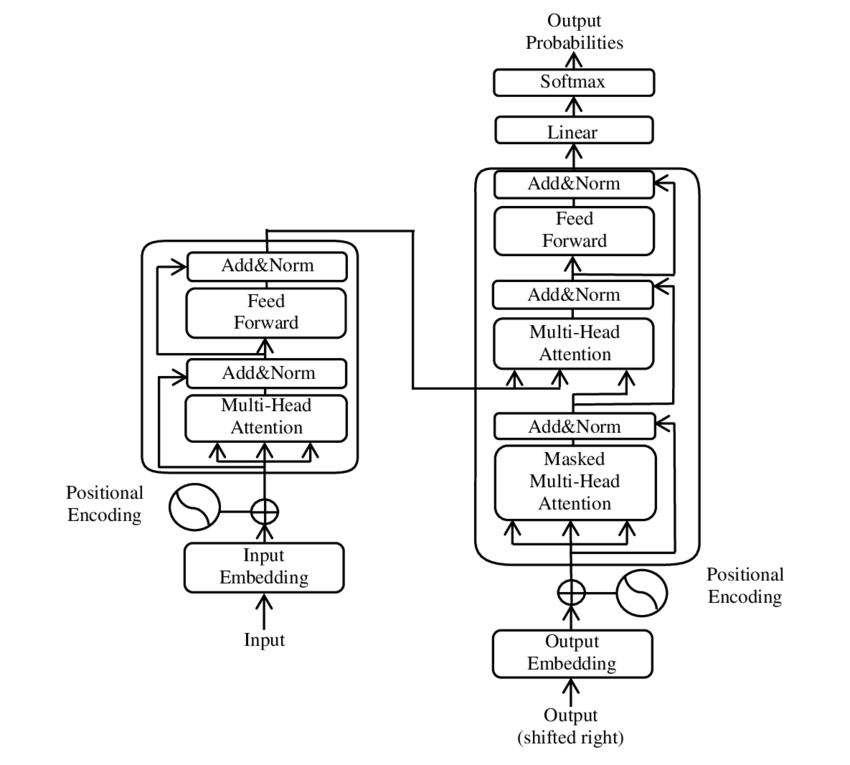
\includegraphics[width=\textwidth]{images/TransformerBlock.png}
\caption{Bloque de transformer}
\label{transformer}
\end{figure}

\newpage

\printbibliography

\end{document}
